% 8.3：依据表6与同源采样场分析收缩过程；图8(a)使用用户更新的PNG，(b)沿用原数据重绘，图9沿用原图。
\subsection{结果分析}
\label{sec:p4-analysis}

结合表\ref{tab:p4C}及图\ref{fig:p4-drying}分析收缩过程，
并通过图\ref{fig:p34-comparison}与固定尺寸工况比较，考察尺寸变化和物性更新的共同影响。

\subsubsection{收缩过程与终点状态}

图\ref{fig:p4-drying}(a)中的黑色曲线表示实际表面$r=R(t)$，
其下方为当时的药材区域。
$6\ \mathrm{h}$时半径已由$2.000\ \mathrm{cm}$降至$1.374\ \mathrm{cm}$，
$36\ \mathrm{h}$时接近$1.200\ \mathrm{cm}$，但中心含水率仍为$0.1928\cunit$。
这表明收缩主要发生在前期，尺寸趋稳早于全域达标，不能以半径趋稳判断干燥结束。

\begin{figure}[!htbp]
\centering
% 保持原图8的0.98\textwidth宽度及275.6785/636.93875高宽比。
% (a)分开裁剪主图、标题与色条；结束时间移至轴框内右上方空白处，避免与色条标题重叠。
% 各部分仅指定一个缩放尺寸，保持原始比例；trim按(a)源PNG的300 dpi换算。
% (b)沿用原始数据，以宋体及Times New Roman重绘，保留原大小与位置。
\setlength{\unitlength}{0.98\textwidth}
\begin{picture}(1,0.432817912)
  % (a)水分场、表面曲线及坐标轴。
  \put(-0.001114244,0.008490525){\makebox(0,0)[lb]{%
    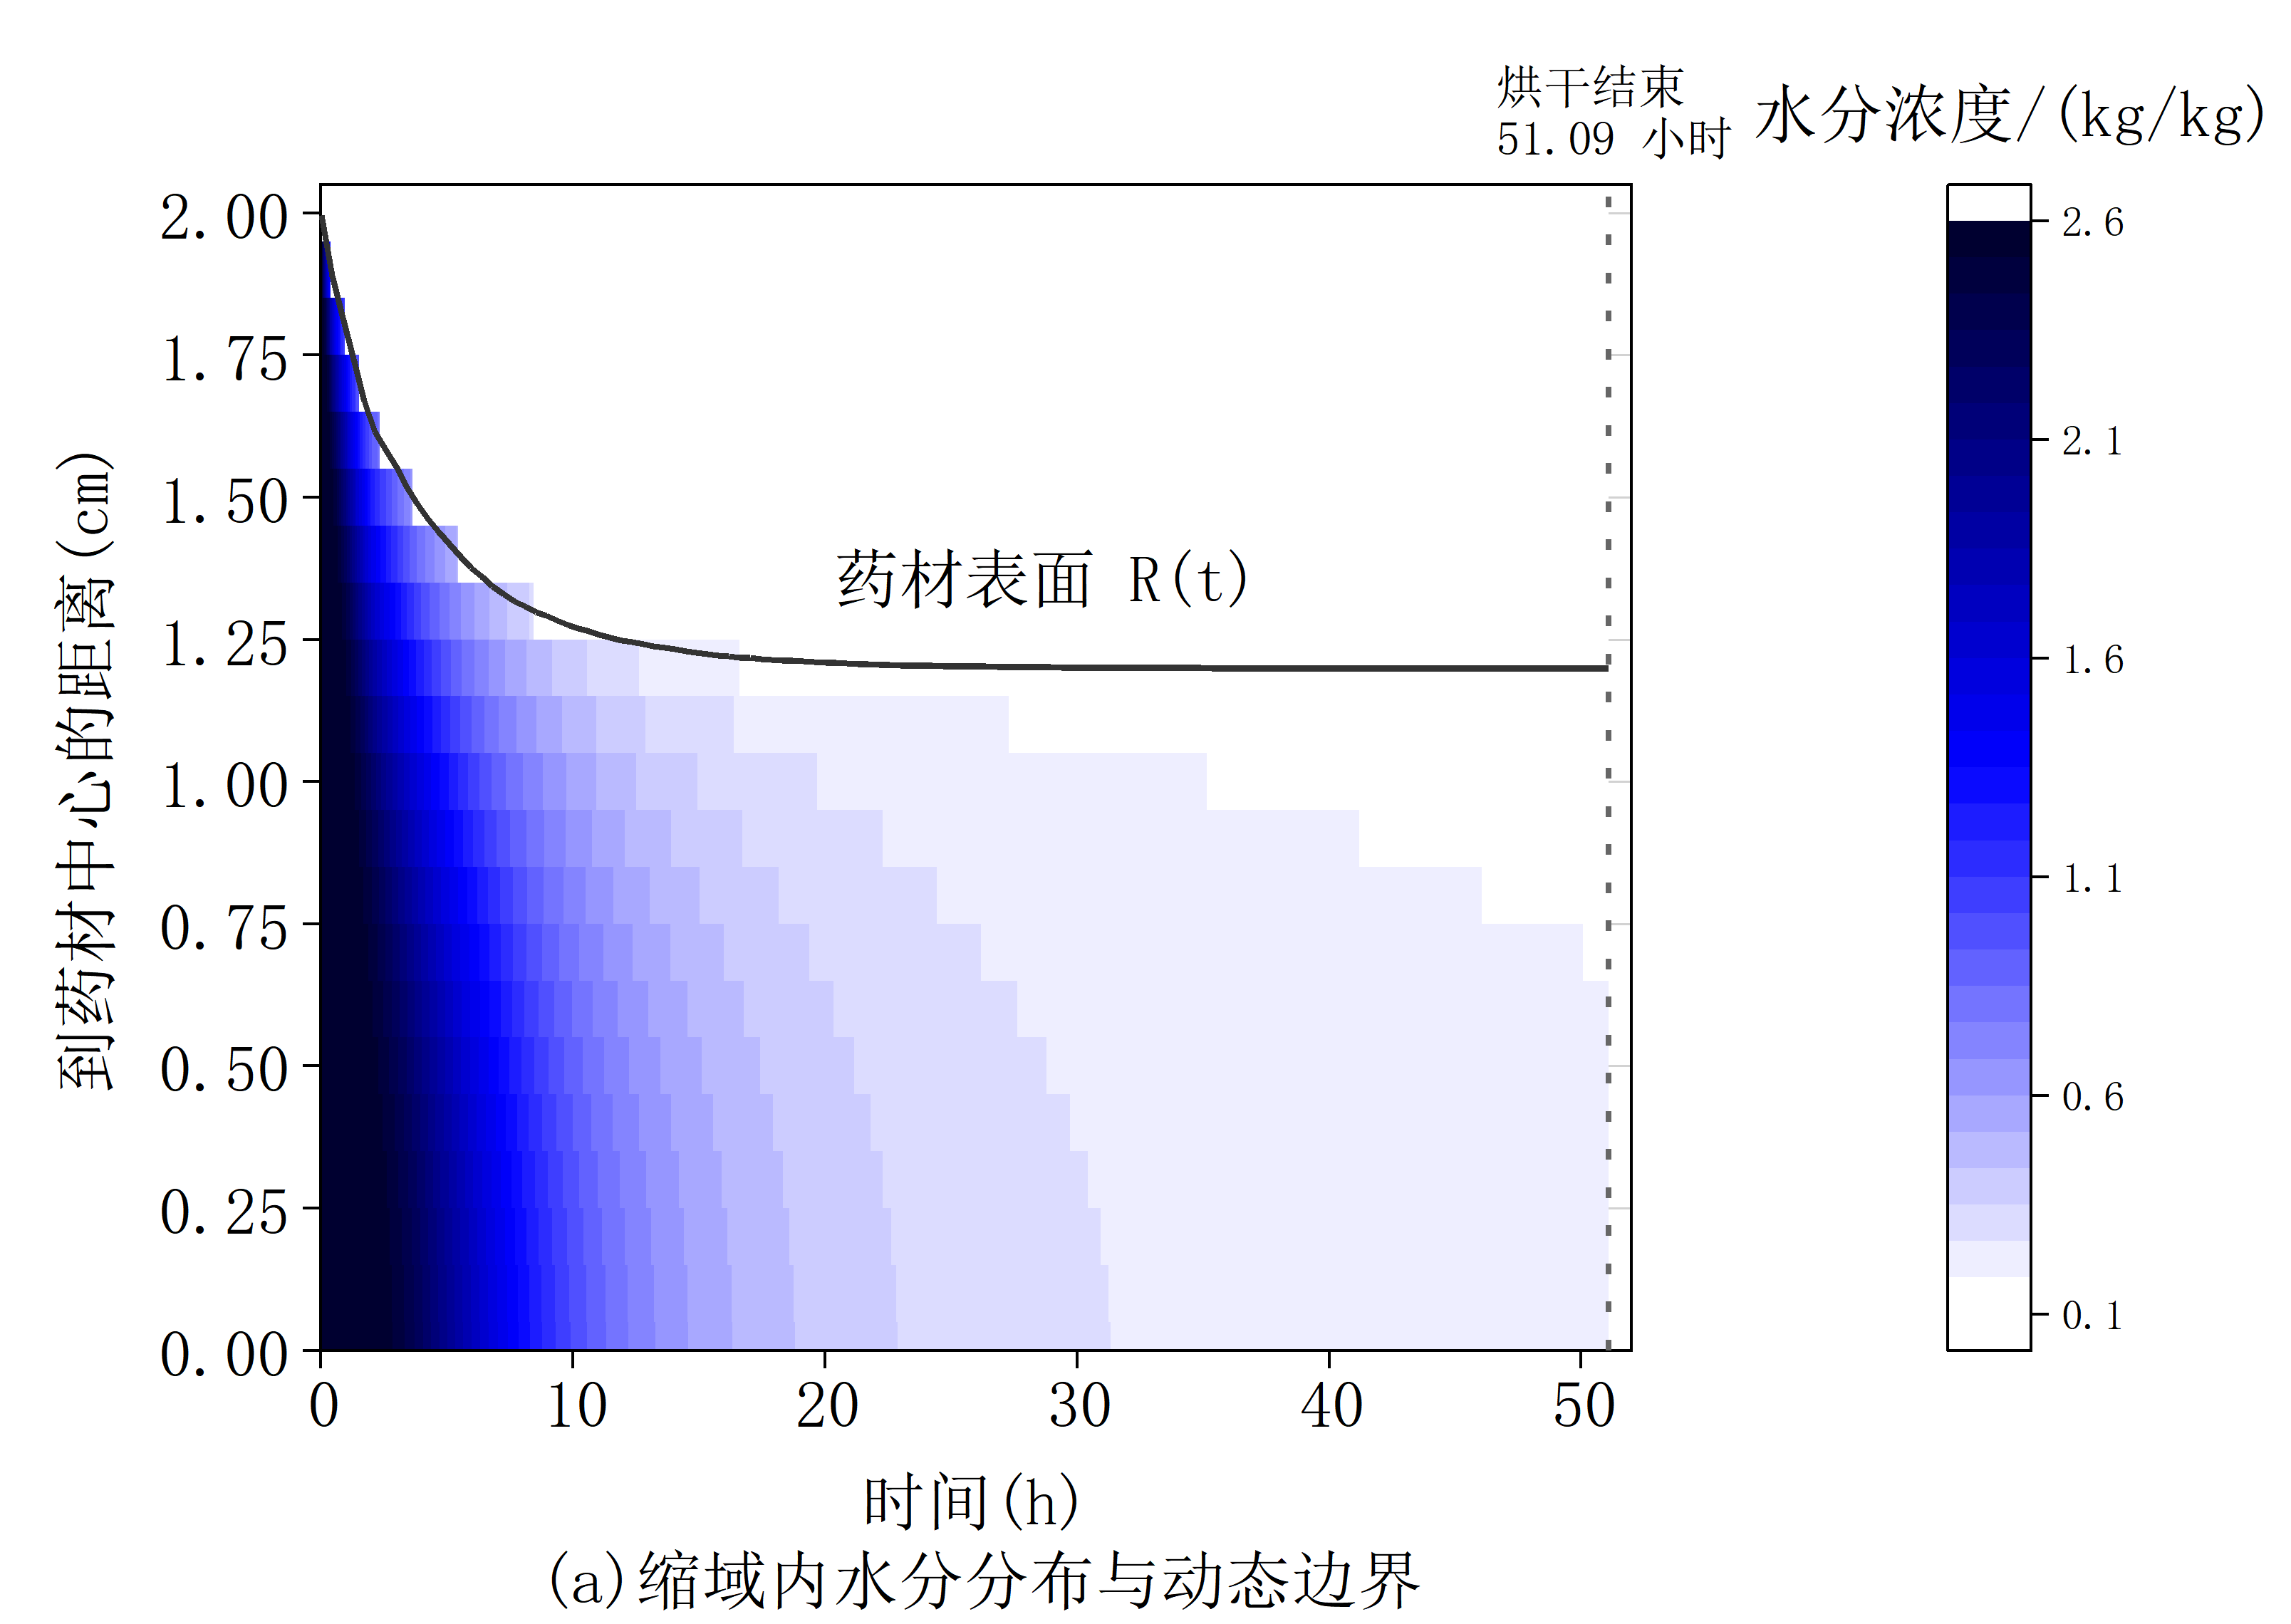
\includegraphics[trim={14.400bp 27.600bp 212.640bp 58.800bp},clip,
      height=0.387954163\unitlength]{图10(a).png}}}
  \put(0.074658053,0.395434391){\makebox(0,0)[lb]{%
    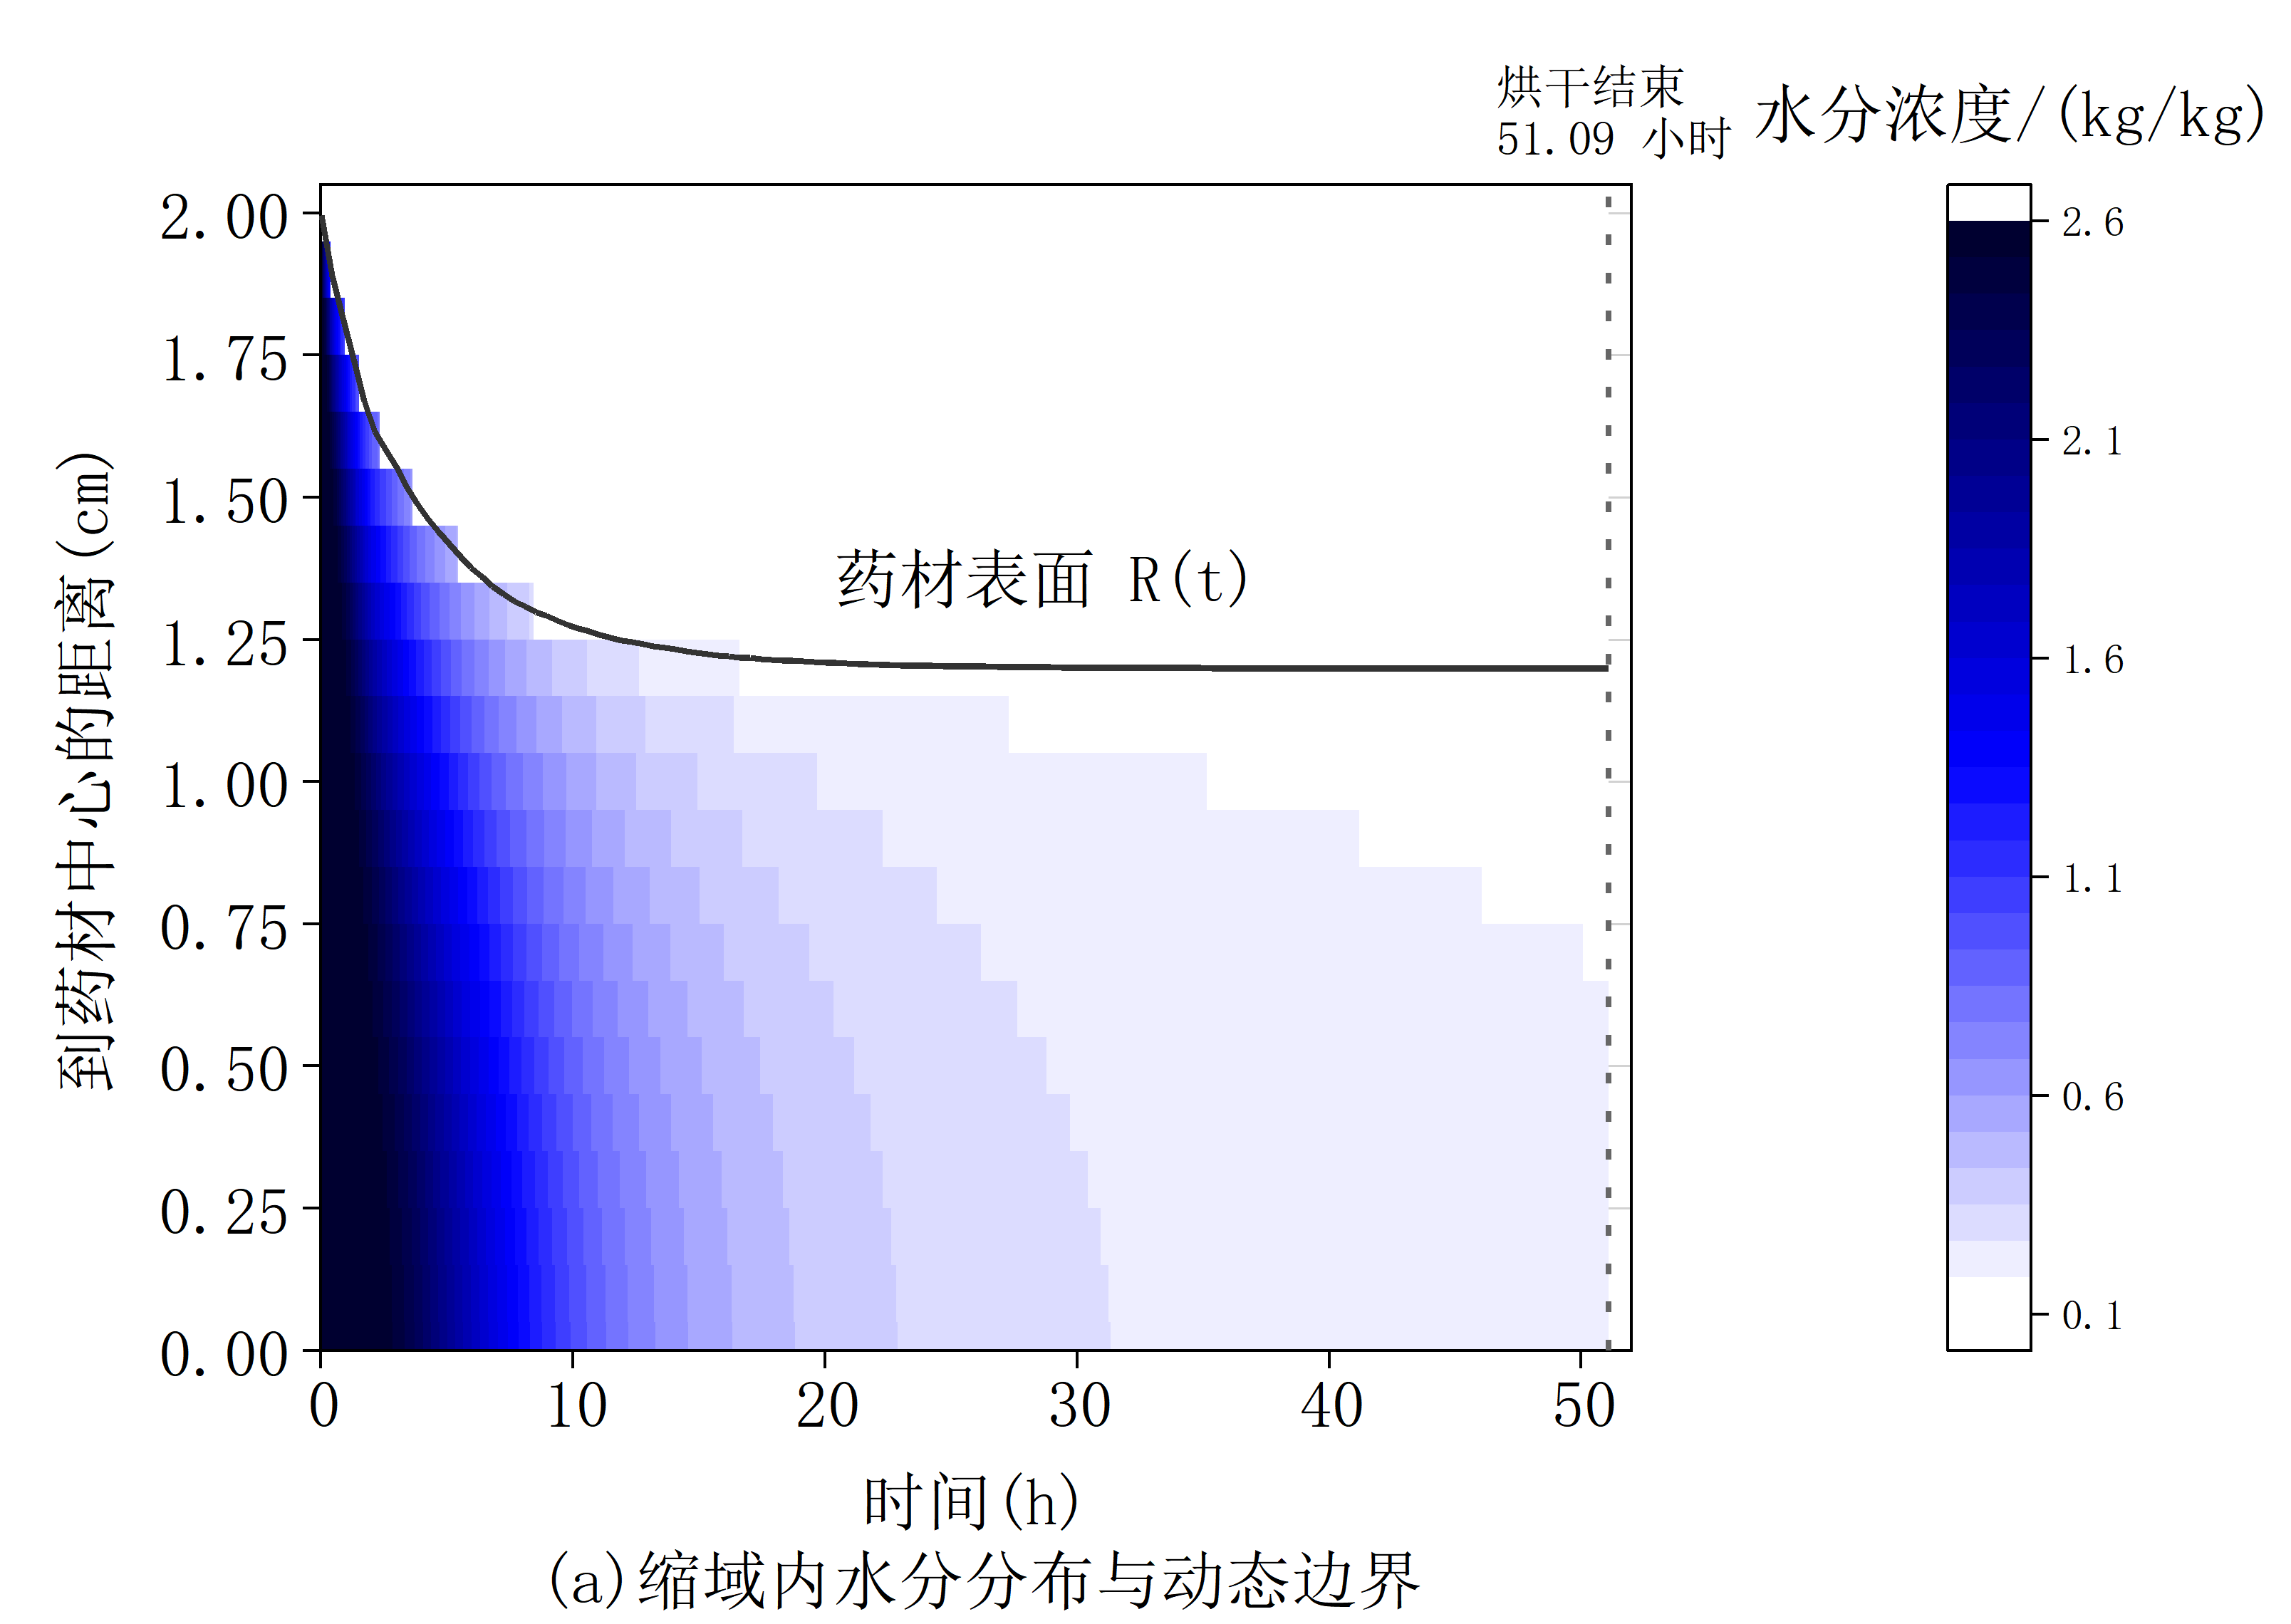
\includegraphics[trim={104.400bp 487.200bp 367.440bp 34.800bp},clip,
      height=0.021216243\unitlength]{图10(a).png}}}
  % (a)色条及单位。
  \put(0.461073868,0.060015687){\makebox(0,0)[lb]{%
    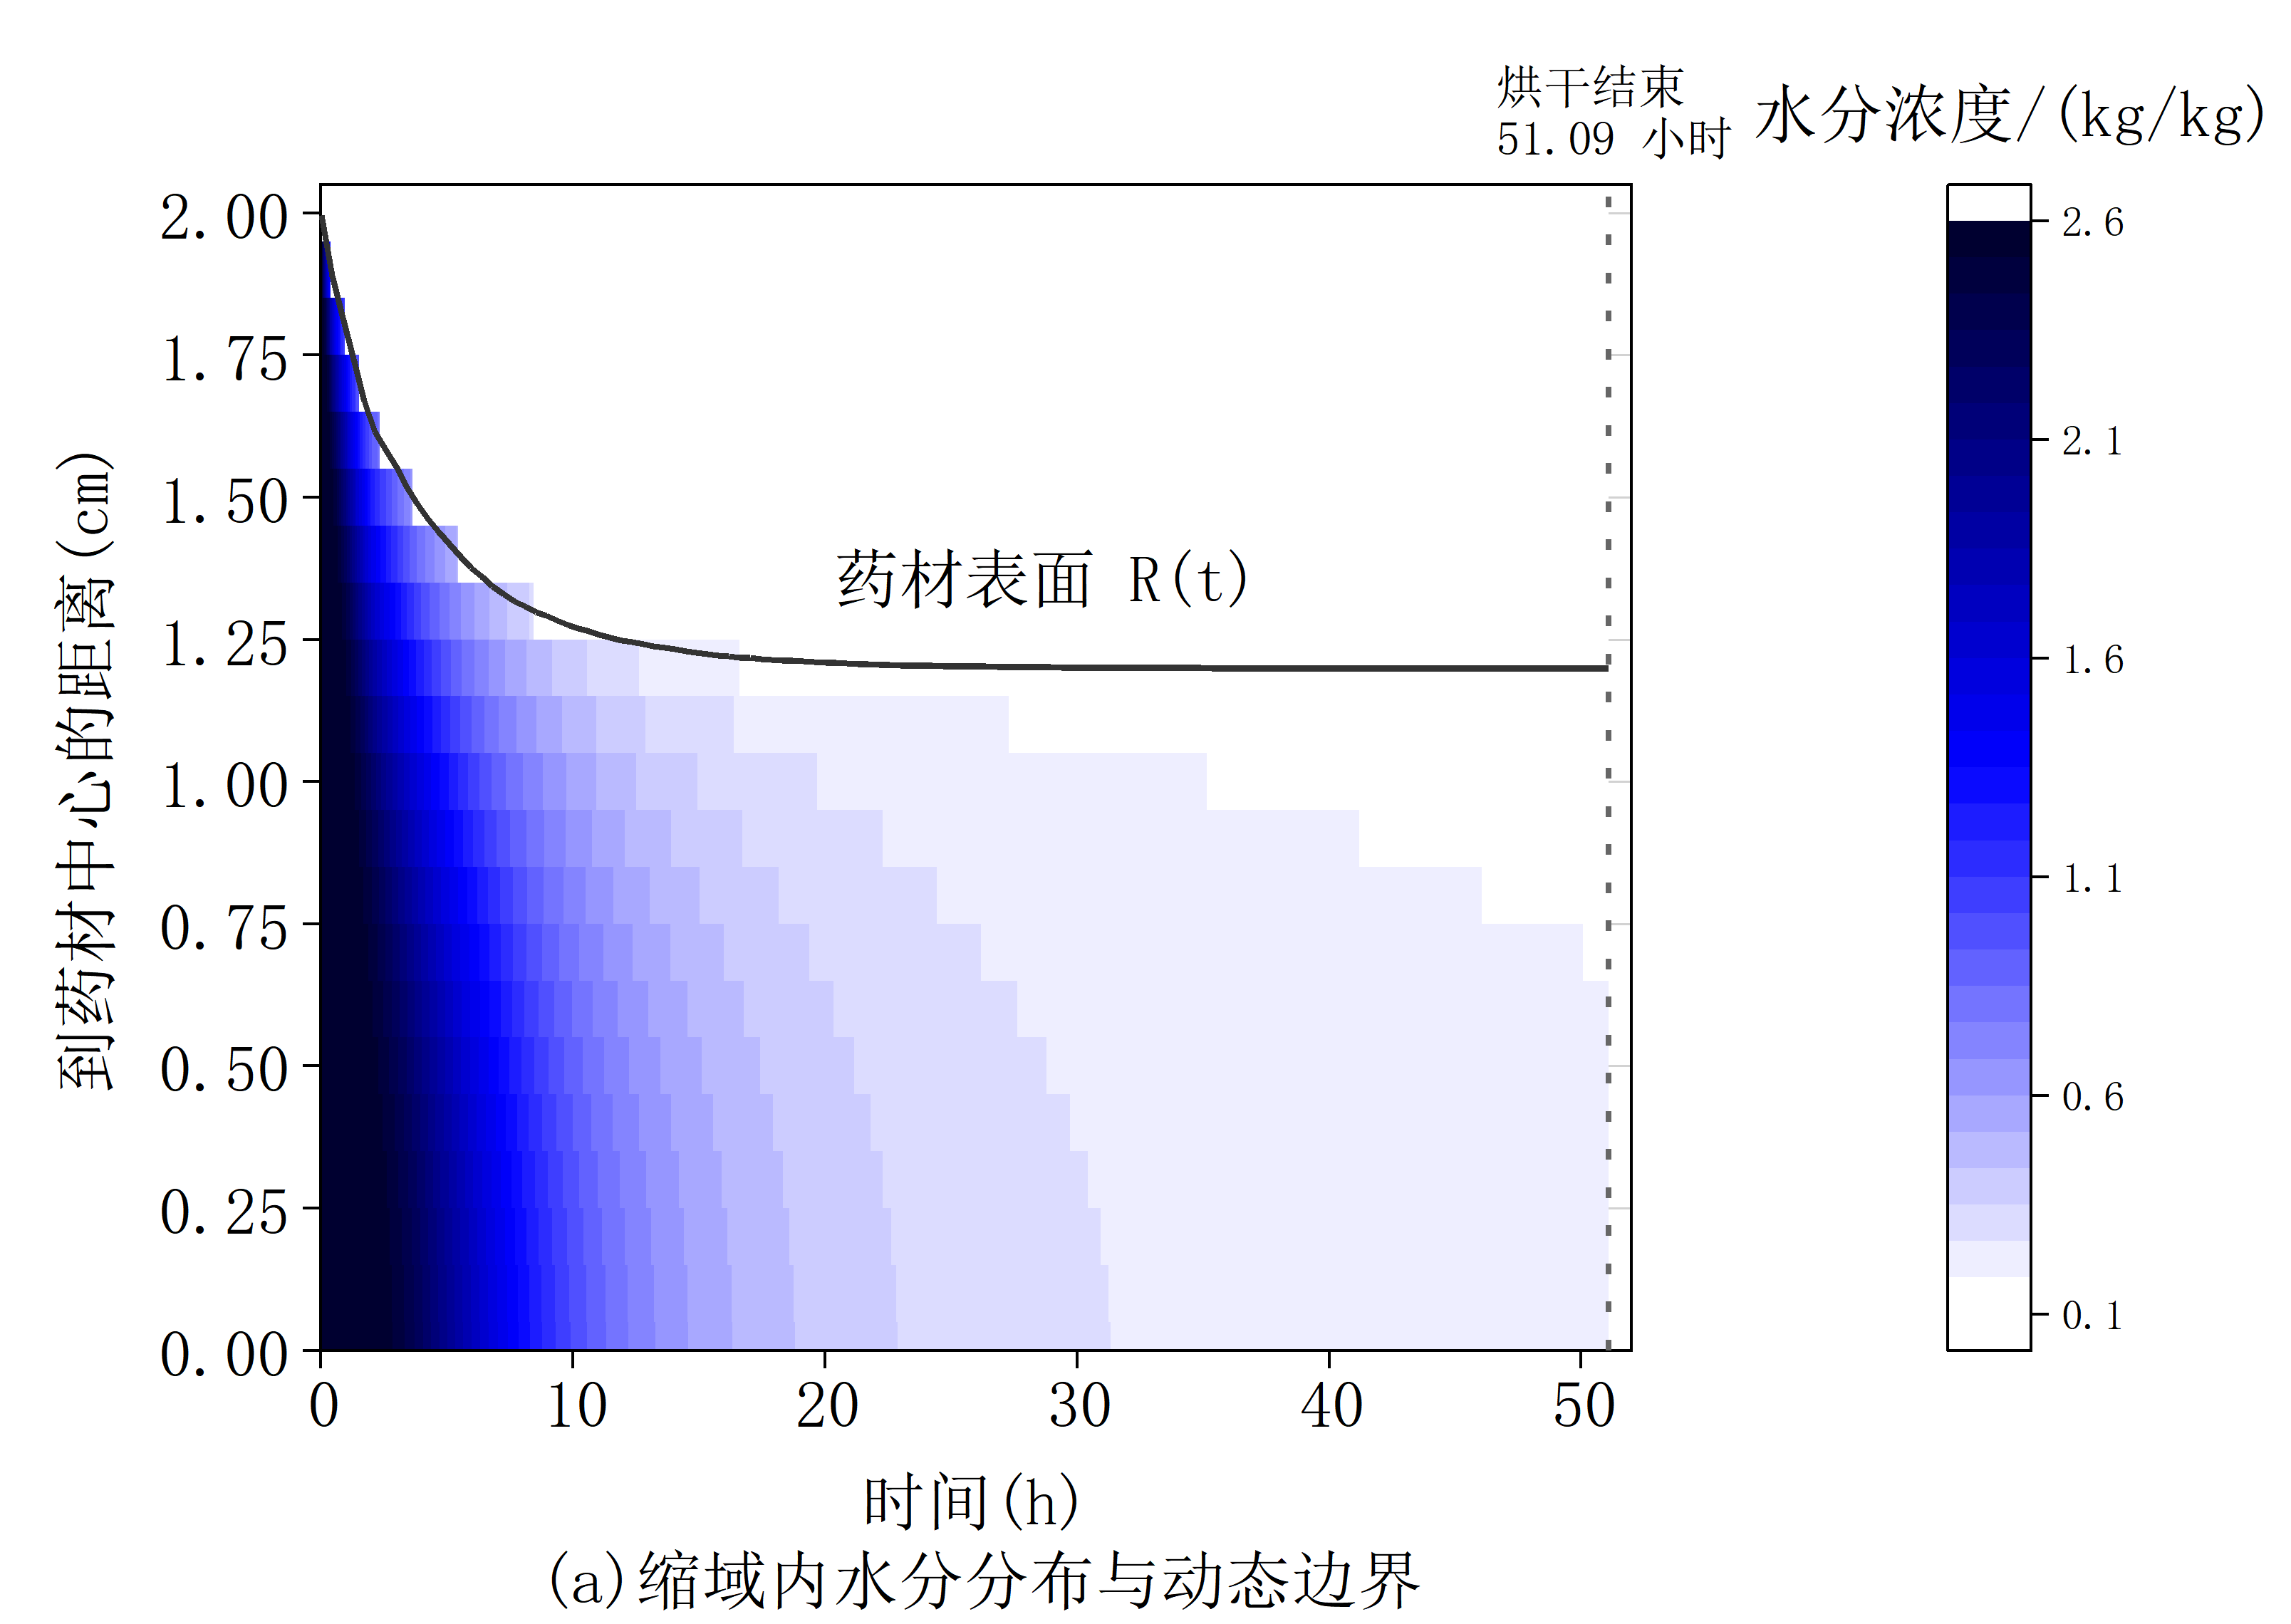
\includegraphics[trim={651.600bp 88.800bp 24.240bp 58.800bp},clip,
      height=0.336429001\unitlength]{图10(a).png}}}
  \put(0.396278884,0.402506472){\makebox(0,0)[lb]{%
    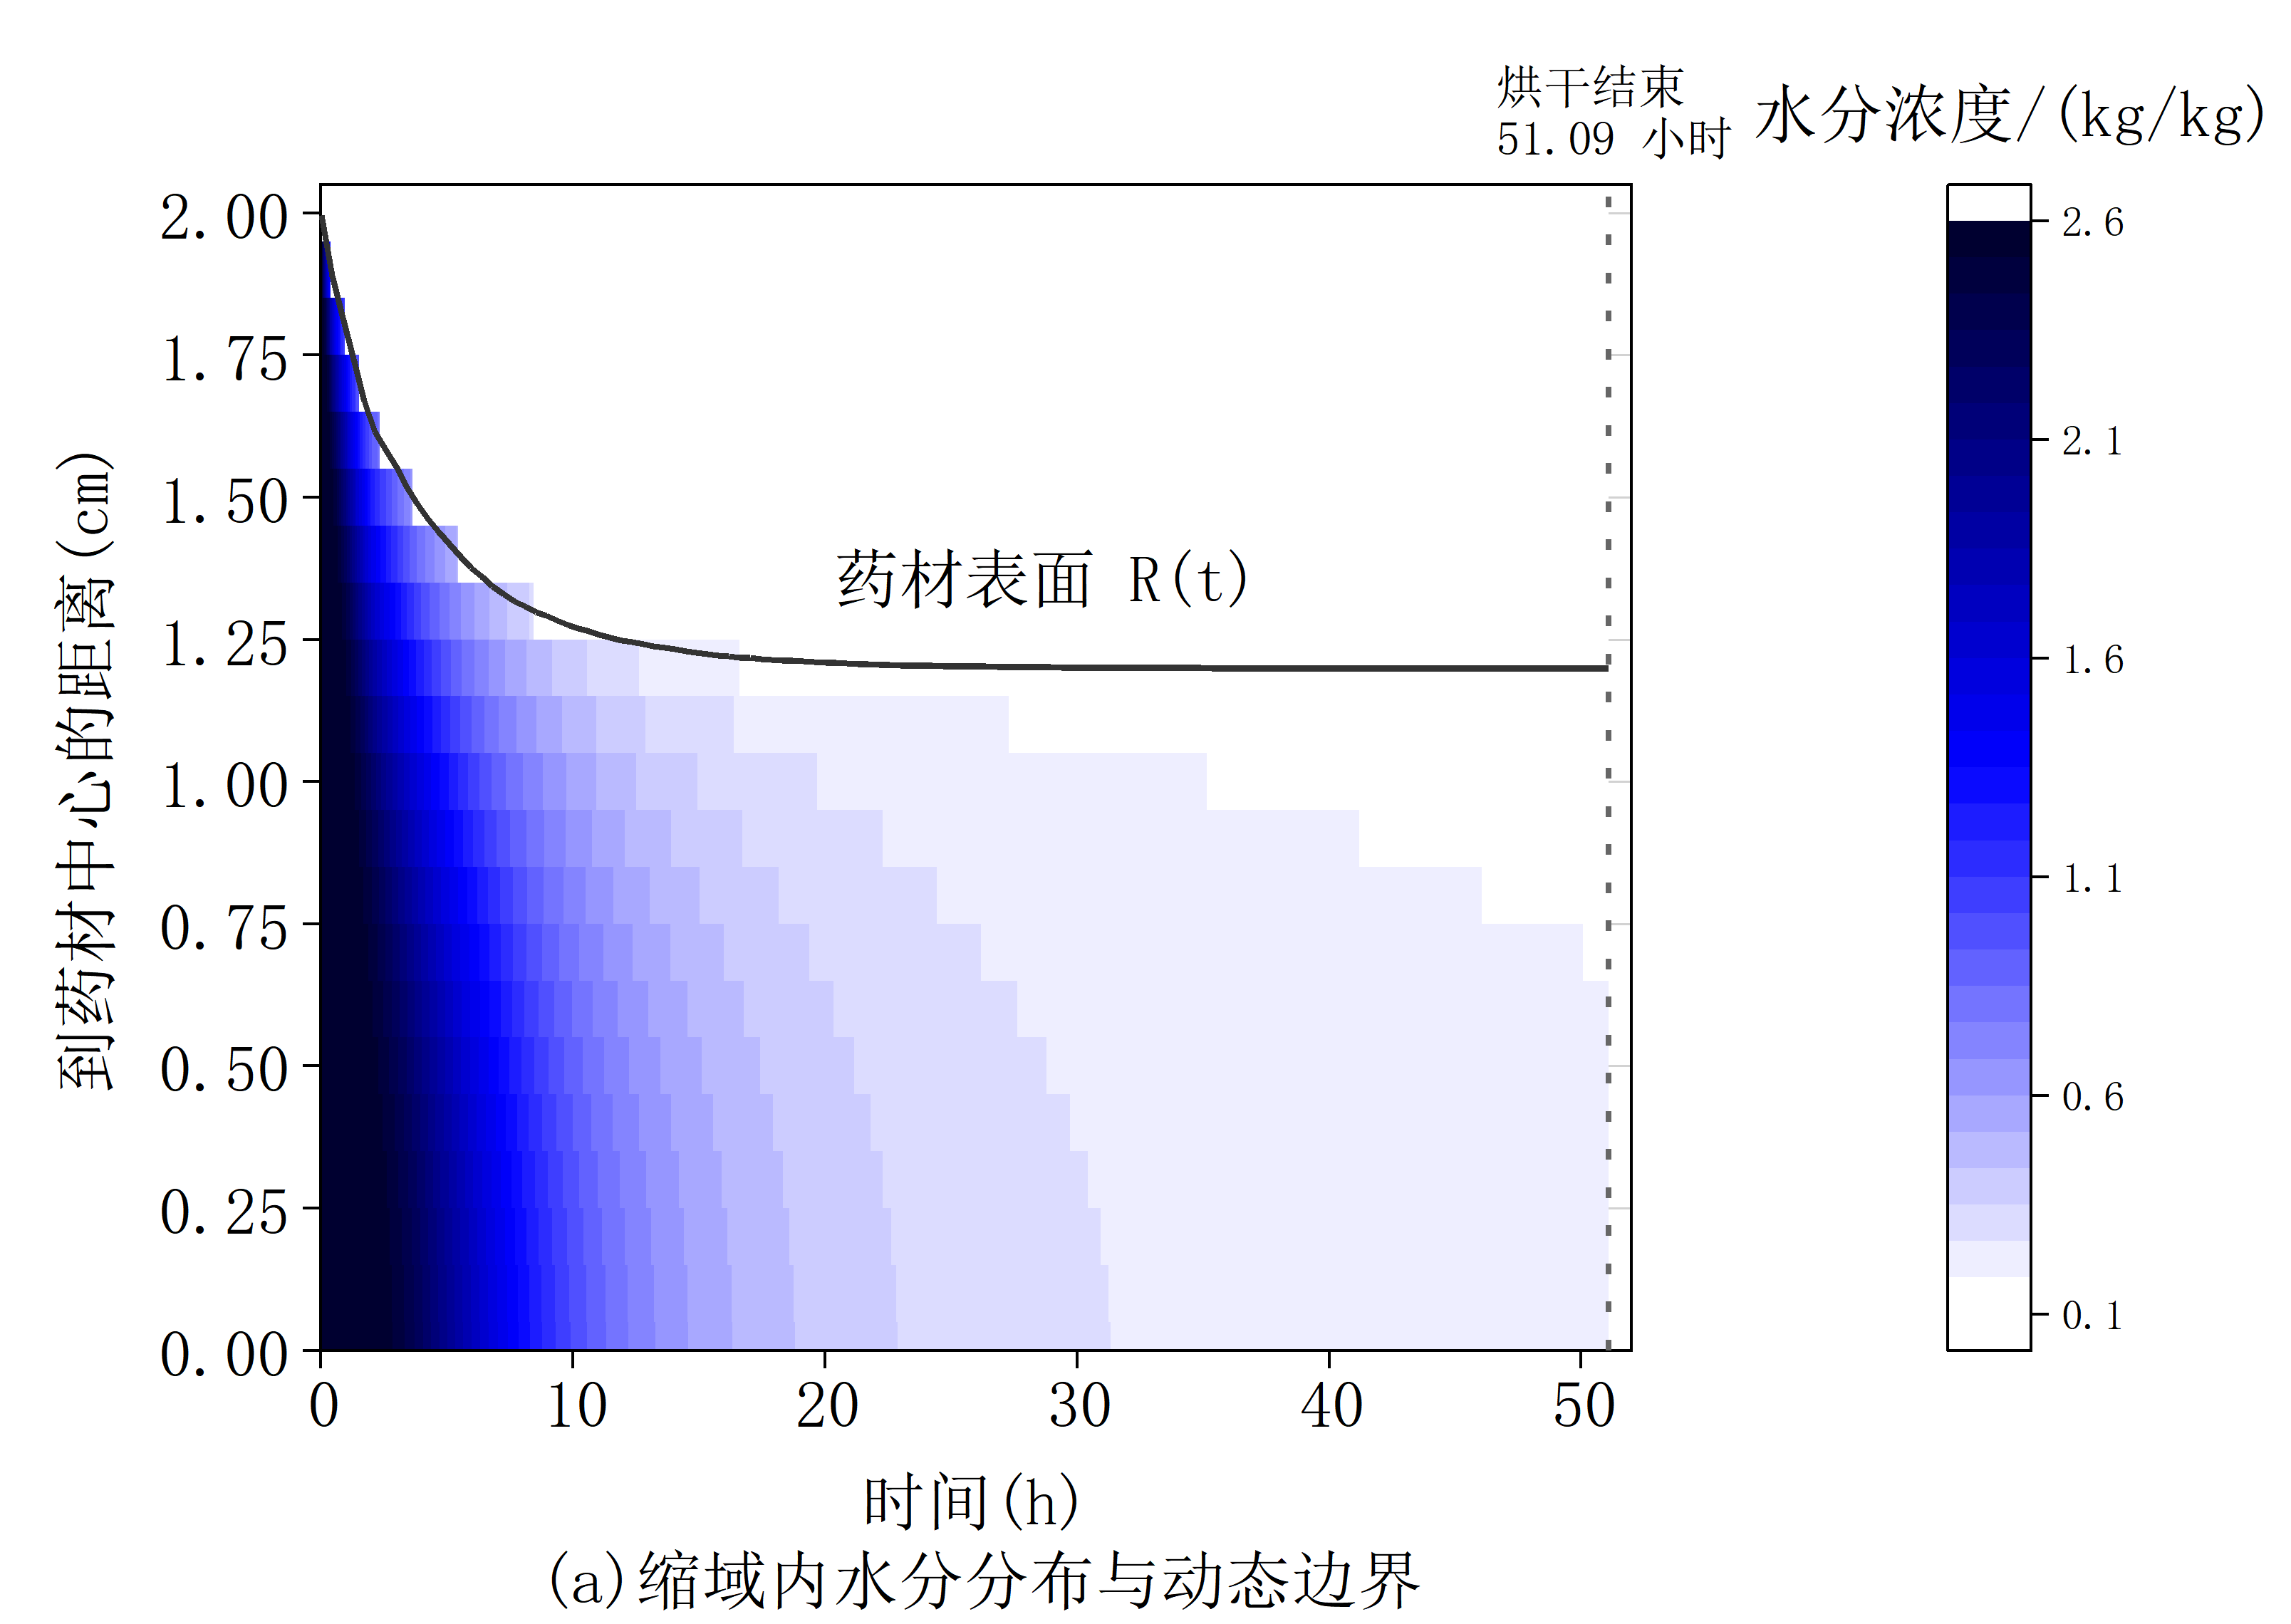
\includegraphics[trim={588.000bp 495.600bp 6.240bp 25.200bp},clip,
      height=0.022226541\unitlength]{图10(a).png}}}
  % (a)完整保留结束时间标注。
  \put(0.370318457,0.339440365){\makebox(0,0)[lb]{%
    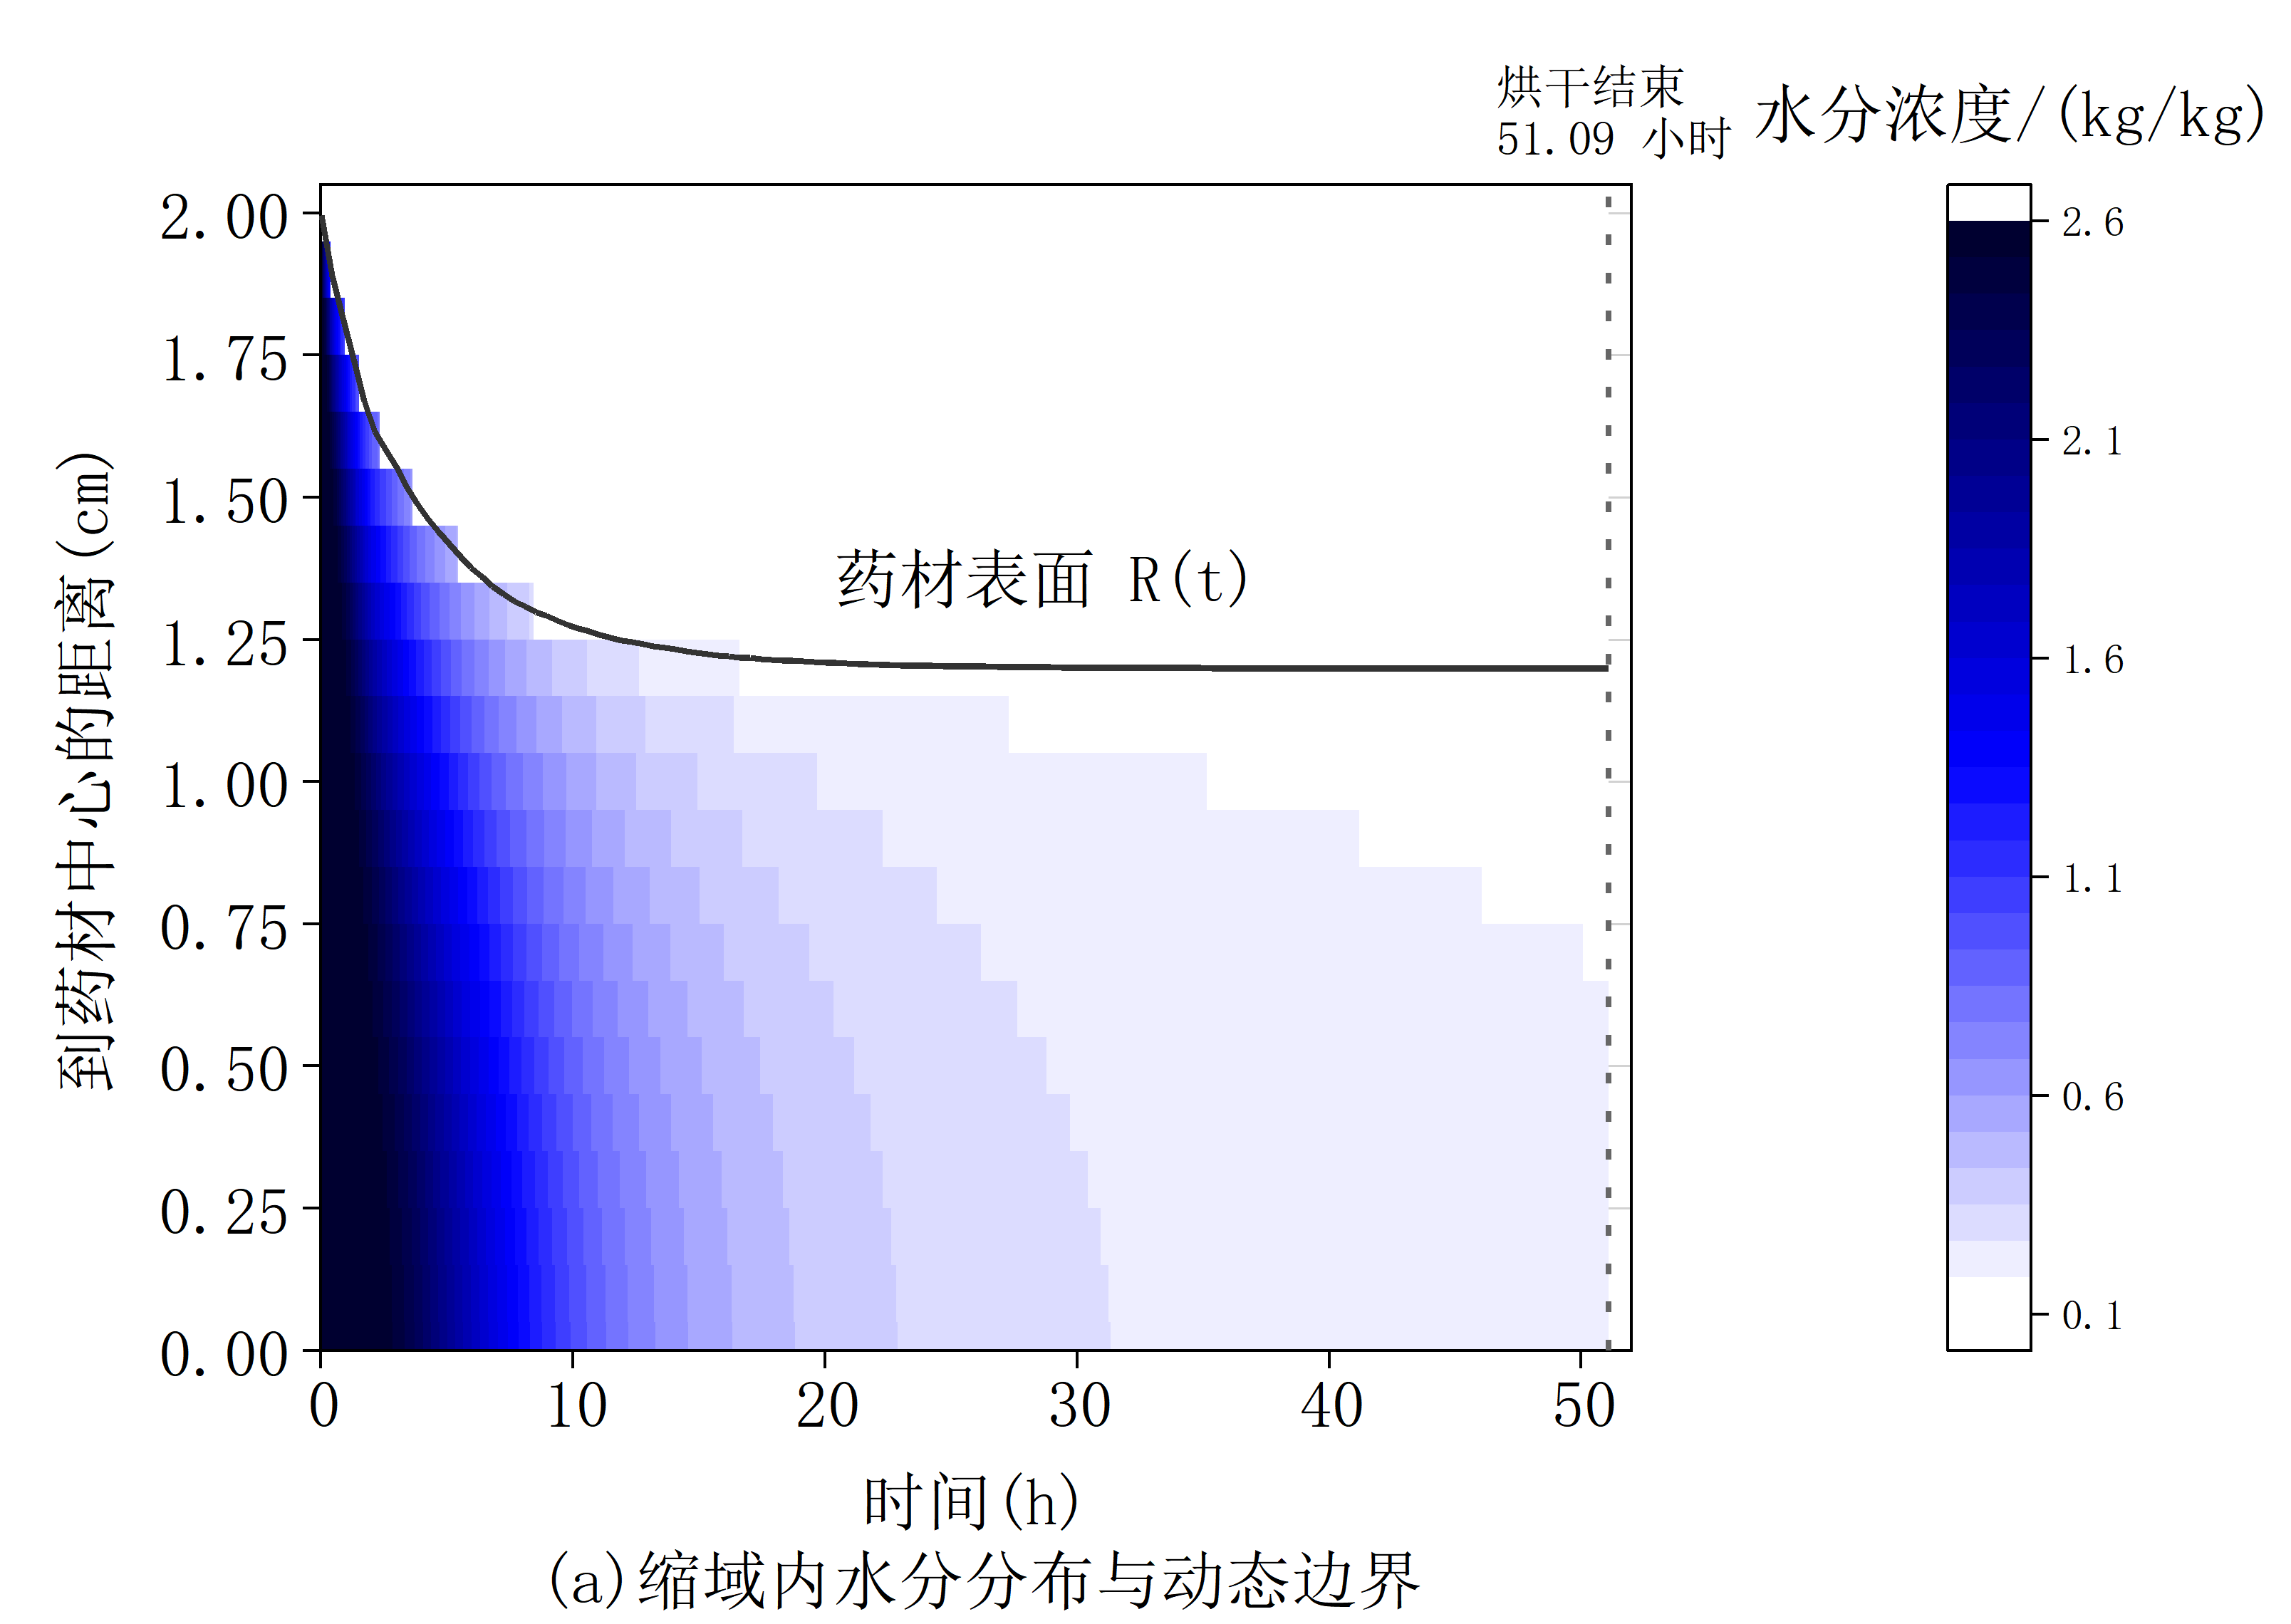
\includegraphics[trim={500.400bp 490.800bp 185.040bp 18.000bp},clip,
      height=0.032329514\unitlength]{图10(a).png}}}
  % (b)半径与平均含水率两幅原有曲线。
  \put(0.549566187,-0.000127956){\makebox(0,0)[lb]{%
    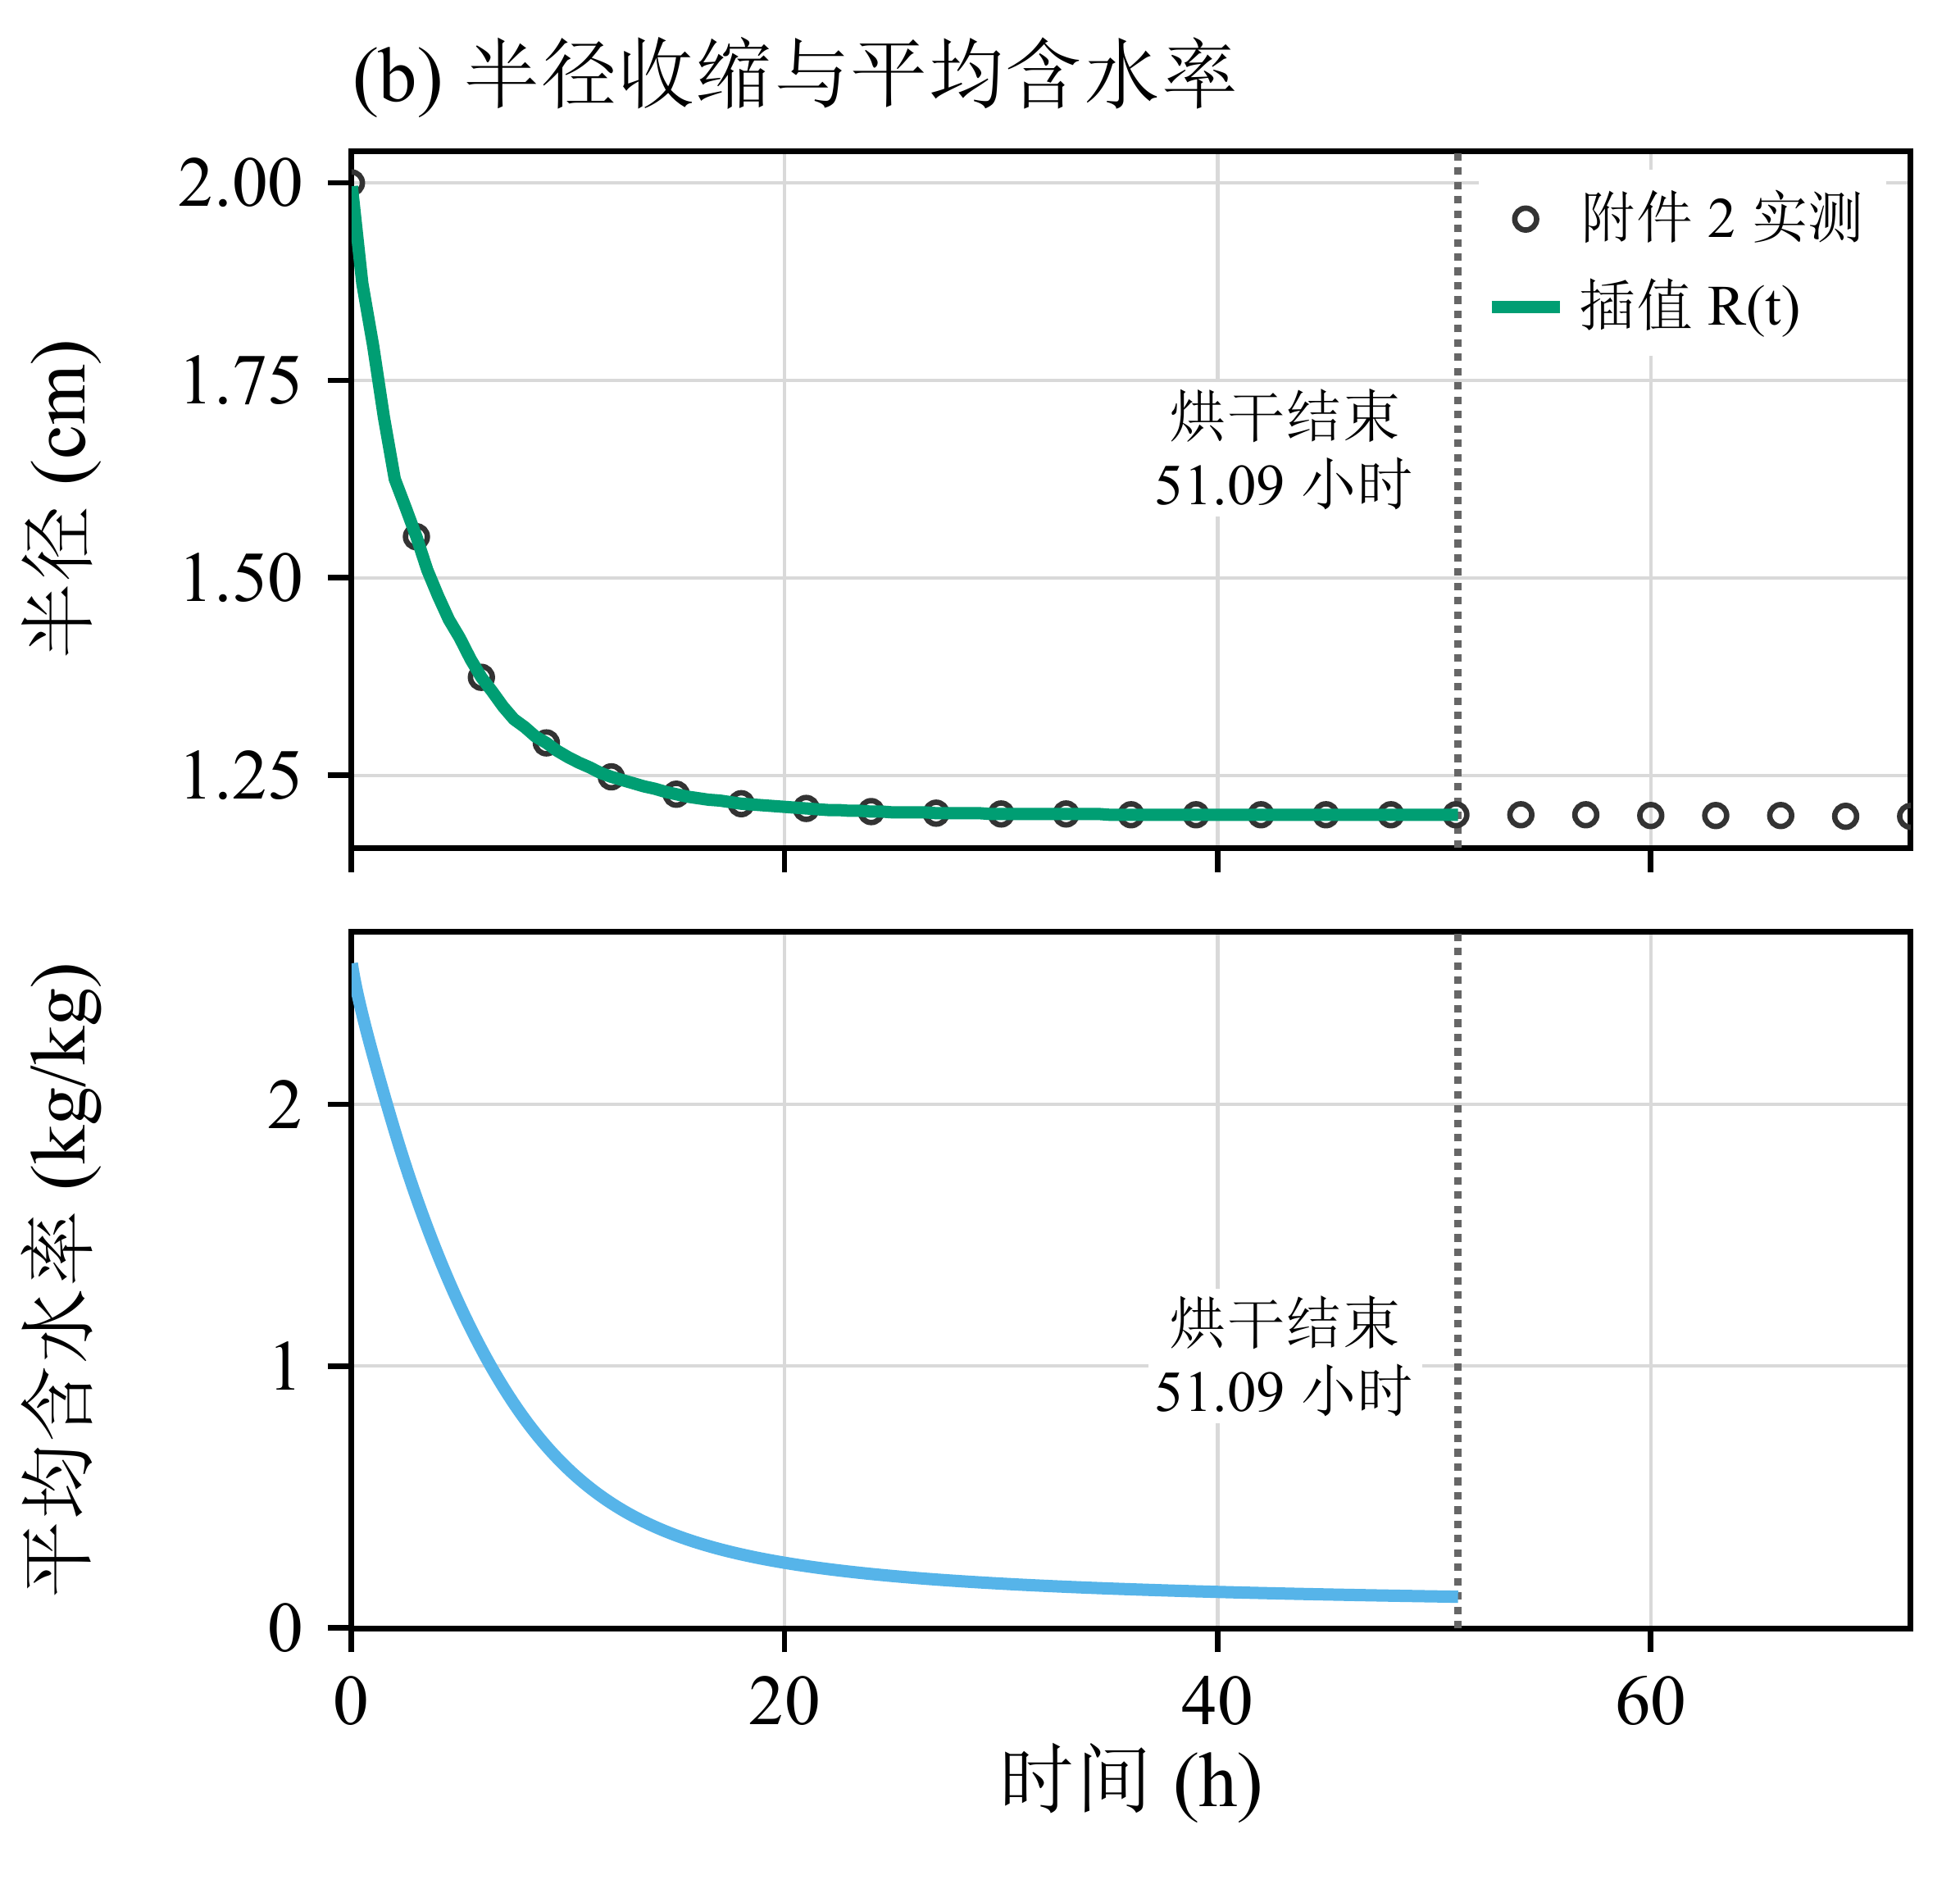
\includegraphics[width=0.450467176\unitlength]{图10(b).png}}}
\end{picture}
\caption{问题四收缩区域内的含水率分布、半径与平均含水率演化}
\label{fig:p4-drying}
\end{figure}

图\ref{fig:p4-drying}(b)中的半径曲线由附件2记录插值得到，属于模型输入；
截面平均含水率按当前截面面积加权，反映给定收缩历程下的计算响应。
半径曲线与记录点吻合不构成对含水率预测的独立验证。

$51.0905\ \mathrm{h}$的临界状态下，中心与实际表面的含水率分别为
$0.1500\cunit$和$0.0526\cunit$，仍存在内湿外干的径向差异。
结合第\ref{sec:p4-solution}节的逐节点核验，本算例仍由中心控制终点。
图\ref{fig:p4-drying}(b)中平均含水率曲线后期趋平，
说明收缩并未消除低含水率阶段的缓慢脱水特征。

\subsubsection{与固定尺寸工况的比较}

本问较问题三的$57.4721\ \mathrm{h}$缩短$6.3816\ \mathrm{h}$，约$11.10\%$。
但图\ref{fig:p34-comparison}中两问的中心含水率曲线约在$41.20\ \mathrm{h}$才交叉：
问题四前期中心含水率较高，此后才更低并率先达标。
因此，总时长较短并不意味着全过程失水更快。

\pfig{图11.pdf}{0.86}{问题三与问题四的中心含水率比较（分别采用附录3、4的物性关系）}{fig:p34-comparison}

以$D_3$、$D_4$分别表示两问的扩散系数。
由式\eqref{eq:p2-properties}、式\eqref{eq:p4-properties}，在相同含水率和温度下有
\begin{equation}
  \frac{D_4(C,T_K)}{D_3(C,T_K)}
    =0.175\exp\!\left(\frac{0.15}{C}\right).
  \label{eq:p34-diffusivity-ratio}
\end{equation}
当$C=1\cunit$和$C=0.0526\cunit$时，该比值分别约为$0.2033$和$3.03$。
附录4在较高含水率下给出的扩散能力较弱，在较低含水率下则较强，
为两问前后期表现的差异提供了物性方面的解释。

同时，问题四临界半径约为初值的$60\%$，缩短了水分迁移距离。
相关文献研究研究也表明，收缩可通过缩短迁移路径加快内部水分脱除\cite{radish-shrinkage}。
上述比较仅解释变化趋势，实际时长仍取决于全域温湿分布及表面交换，不能由局部扩散系数直接推定。
两问的热物性也同时改变，故\textbf{时长差反映尺寸收缩与物性更新的共同作用}；
若要单独量化收缩贡献，仍需在相同物性下比较固定与收缩半径两种工况。
